\documentclass[12pt,a4paper]{article}
\usepackage[utf8]{inputenc}
\usepackage{amsmath}
\usepackage{amsfonts}
\usepackage{amssymb}
\usepackage{makeidx}
\usepackage{graphicx}
\usepackage[left=2cm,right=2cm,top=2cm,bottom=2cm]{geometry}

\begin{document}
\title{\textbf{Sistemas electronicos de interfaz\\EV 2.3. Explicar los arreglos y parametros de los amplificadores clase B\\Tarea 4}}
\author{Josue Natanael Orozco Nevares 18311797\\Ing. Mecatronica\\Grado 4B}
\date{8 de octubre del 2019}
\maketitle
\begin{figure}[h!]
\centering

\includegraphics[width=10cm]{UPCDLZMDG5783-logo.png} 
\end{figure}
\newpage

\section{Introducciòn}
En esta investigaciòn indagaremos acerca de los amplificadores clase b, desde sus arreglos hasta sus parametros y averiguar en que nos pueden llegar a servir dependiendo la situaciòn.

\section{Amplificadores de clase B}
Los amplificadores de clase B se caracterizan por tener intensidad casi nula a través de sus transistores cuando no hay señal en la entrada del circuito, por lo que en reposo el consumo es casi nulo. Recordar que la caracteristica principal de estos amplificadores es el alto factor de amplificaciòn que poseen.

\begin{figure}[h!]
\centering
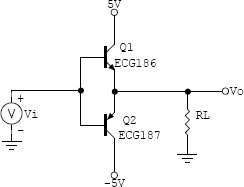
\includegraphics[width=9cm]{AmplificadorClaseB.jpg} 
\end{figure}

\section{Caracteristicas}
Se les denomina amplificador clase B, cuando el voltaje de polarización y la máxima amplitud de la señal entrante poseen valores que hacen que la corriente de salida circule durante el semiciclo de la señal de entrada.\\Dado que ocupa un lugar intermedio entre los de clase A y AB, cuando el voltaje de la señal es moderado funciona como uno de clase A, cuando la señal es fuerte se desempeña como uno de clase B, con una eficiencia y deformación moderadas.

\section{Ventajas}
Posee bajo consumo en reposo.\\Aprovecha al máximo la Corriente entregada por la fuente.
\\Intensidad casi nula cuando está en reposo.

\begin{figure}
\centering
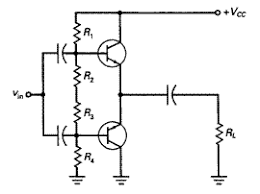
\includegraphics[width=5cm]{AmplificadorClaseB2.png} 
\end{figure}

\section{Desventajas}
Este tipo de amplificadores producen armonicos, y es mayor cuando no tienen los transistores de salida con las mismas características técnicas, debido a esto se les suele polarizar de forma que se les introduce una pequeña polarización directa. Con esto se consigue desplazar las curvas y se disminuye dicha distorsión.

\section{Conclusiòn}
En base a la investigaciòn se descubrio que este tipo de amplificadores nos funcionan para amplificar la señal sin temor a que este mismo consuma energia aun estando en reposo, tambien se descubrio que este tipo de amplificadores se utilizan en sistemas telefonicos, sistemas de avisos pero sin salida de audio o inclusive en transmisiones de seguridad.


\end{document}